Feedback-driven speech recognition repeatedly turns generated text into
input for later inference. A trusted correction can improve the current
transcript and change the state from which the next recognition starts.
This makes each correction an execution boundary: some ongoing speculative
work has become invalid, while other work may still be a valid continuation.
A dependable service must distinguish these cases while delivering useful
progress before its trusted path catches up.

An execution from our prototype exposes the problem. A complete hypothesis
covering a two-second audio interval reached the actual Consumer 1.444~s
after that interval became available, meeting its two-second display
deadline. At 1.544~s, a new certified result replaced the visible view with
a shorter snapshot. The discarded hypothesis still had a valid dependency
path from the new feedback state. It remained absent at the original
two-second deadline and returned at 3.720~s through certified delivery,
within its eight-second deadline and with exactly the same text. The
temporary loss removed 37 newly displayed characters, including spaces.
Both first-delivery deadlines were met, yet already delivered valid progress disappeared for
2.176~s. This is a loss of interval coverage under a compatible update,
independent of whether the provisional transcription is semantically correct.

\begin{figure*}[t]
\centering
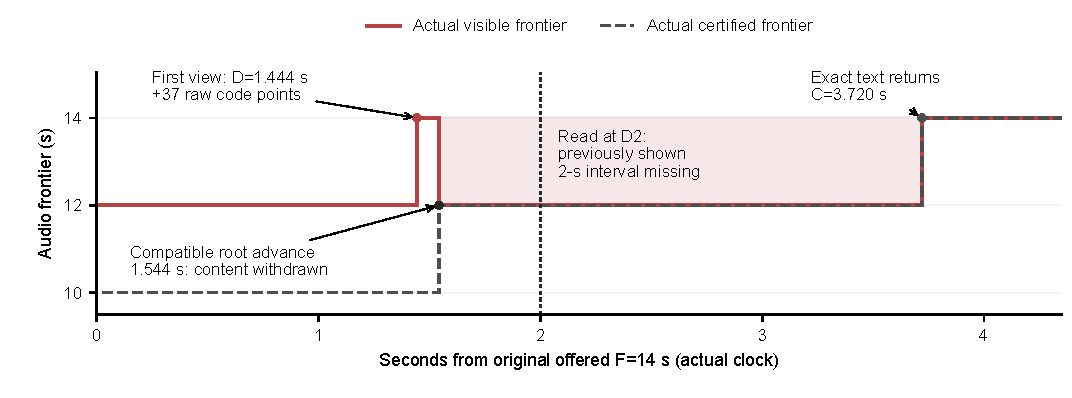
\includegraphics[width=\textwidth]{figures/timely_full_interval_case.pdf}
\caption{An actual interval in the computation-only arm. First display meets
D2 and certified delivery meets C8, yet a compatible root update withdraws
the newly displayed phrase for 2.176~s. The dotted line samples the actual
view at the original D2 deadline. This explanatory case comes from the
c16 workload, whose whole-run D2 P99 fails; it is not a paired
counterfactual or an estimate of natural prevalence.}
\label{fig:continuity_case}
\end{figure*}

Computation retention alone can exacerbate this mismatch. In our
predeclared Qwen evaluation on three new eight-speaker cohorts, retaining
valid computation improved timely delivery but increased observed
audio-frontier withdrawals from 12 to 17 when the Consumer still installed
snapshots. Retaining the computation and its compatible whole view together
produced zero frontier withdrawals in that stratum. The issue is therefore
how valid work becomes sustained service across a trusted update, as well
as how quickly the work finishes.

There are strong foundations for this design. Incremental dialogue models
already distinguish active and committed information and propagate
revocation~\cite{schlangen2011incremental}; incremental computation reuses
work through dependencies and stable identities
\cite{hammer2014adapton,hammer2015names,mcsherry2013differential}.
SSBD coordinates old draft reuse with display-only masking in
re-translation~\cite{zeng2026ssbd}, and PredGen speculates on downstream
responses while speech input evolves~\cite{li2025predgen}. We apply these
ideas to a protected feedback contract in which the original trusted
selection recursively supplies later ASR inputs. The contract governs two
decisions: whether executed work remains eligible under the new root, and
whether installing that root preserves the Consumer's current whole
hypothesis. Separate sufficient guards enforce the feedback dependencies
at these boundaries. Together they provide conditional continuity of
already delivered progress while retaining selection authority and
necessary revisions.

RevTrace reconciles executed calls and delivered whole hypotheses with each
new trusted feedback state. A call remains eligible when its complete frozen
input has a valid dependency witness from that state; the Consumer separately
checks whether its current whole hypothesis remains supported. These
decisions retain work and service while original protected selection
determines the next feedback state. We instantiate the same eligibility
principle with recorded continuation paths in the core runtime and with
input-confirmed full calls in a native correction pipeline. Work with no
remaining use follows a separate coverage rule, and its physical lease ends
only after actual drain.

This paper makes three contributions:
\begin{itemize}
\item A feedback-state contract and executable sufficient witnesses for
  retaining owned computation across trusted updates, including recorded
  continuations and input-confirmed full calls. These witnesses bind
  complete state, actual audio frontiers, frozen inputs, and execution
  identity.
\item Joint coordination of computation and whole Consumer views, with a
  conditional guarantee that applying a compatible certified root does not
  itself withdraw an ahead view. Necessary revisions remain permitted.
\item An implementation and service evaluation that hold the selected
  feedback task fixed. Factorial controls isolate computation and whole-view
  retention; a published native correction pipeline tests whether
  input-confirmed full execution improves timely service while preserving
  original correction and complete state transitions.
\end{itemize}

In the independent headline stratum, the joint design adds 26.645~s of
original dual-deadline credit over 714.110~s offered audio while preserving
the complete certified histories. A separate 48-run workload study shows
where the arms converge and where deadline pressure remains, including a
negative intermediate-load confirmation. Subsequent-availability analysis
keeps its own definition and leaves the original first-delivery metrics
unchanged. A separately frozen native confirmation on four previously
unused speakers raises credit from 37.0 to all 66.340~s offered per arm
and whole-run D2/C8 passes from zero to eight of eight runs.
The core study isolates whole-view continuity; the native study tests
timely execution of the unchanged original feedback task.
